\setlength{\headheight}{-50pt}
\chapter{Vorlesung}
\vspace{-40pt}
\begin{figure}[H]
\centering
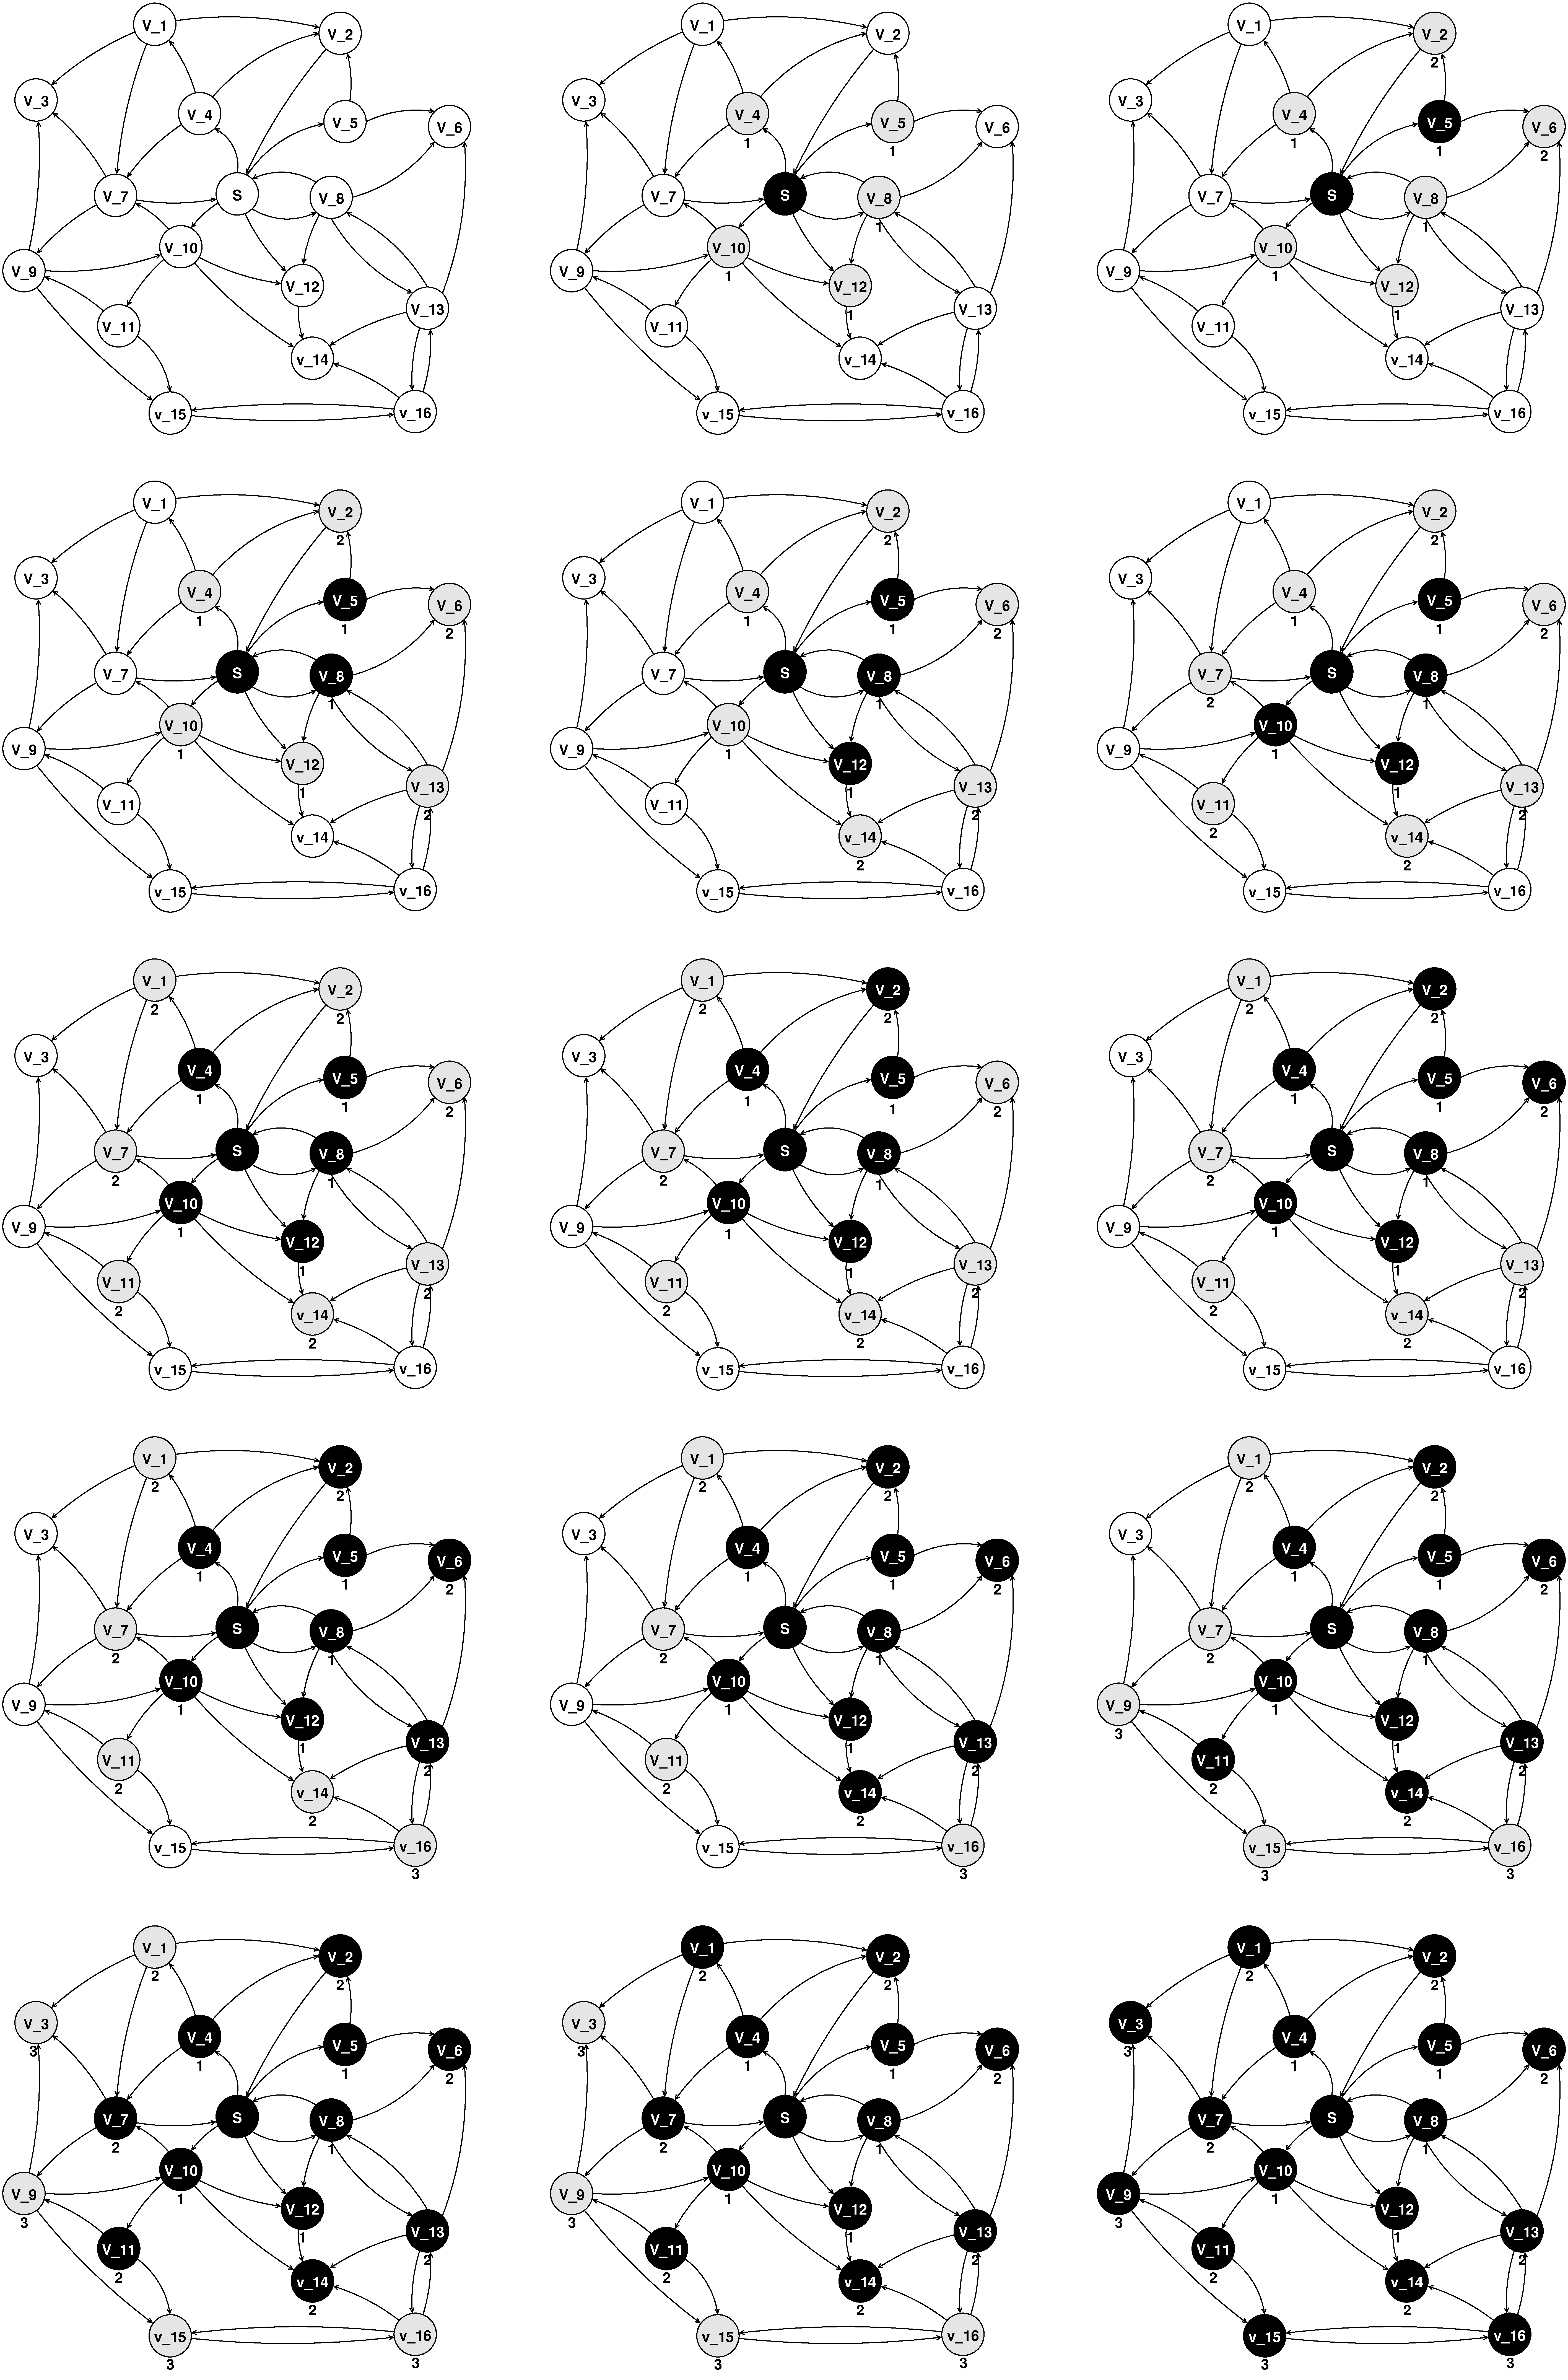
\includegraphics[width=0.9\linewidth]{16/Grafik/Diagramm}
\caption{Beispiel}
\label{fig:Diagramm}
\vspace{-80pt}
\end{figure}
\clearpage
\setlength{\headheight}{0pt}
\subsubsection{Definition: Länge kürzesten Weges}
$\delta(s,v)=$ Länge eines kürzesten Weges vom Startknoten $s$ zum Knoten $v$.\\
Setze $\delta(s,v)=\infty$, falls v nicht erreichbar von s aus.
\subsubsection{Satz: Richtigkeit des Algorithmus}
Nach Ablauf von BFS\footnote{Breitensuche} gilt 
\[ \forall v\in V: ~ d[v]=\delta(s,v) \]
\subsubsection{Lemma 1: Dreiecksungleichung für kürzeste Wege}
\begin{figure}[h]
\centering
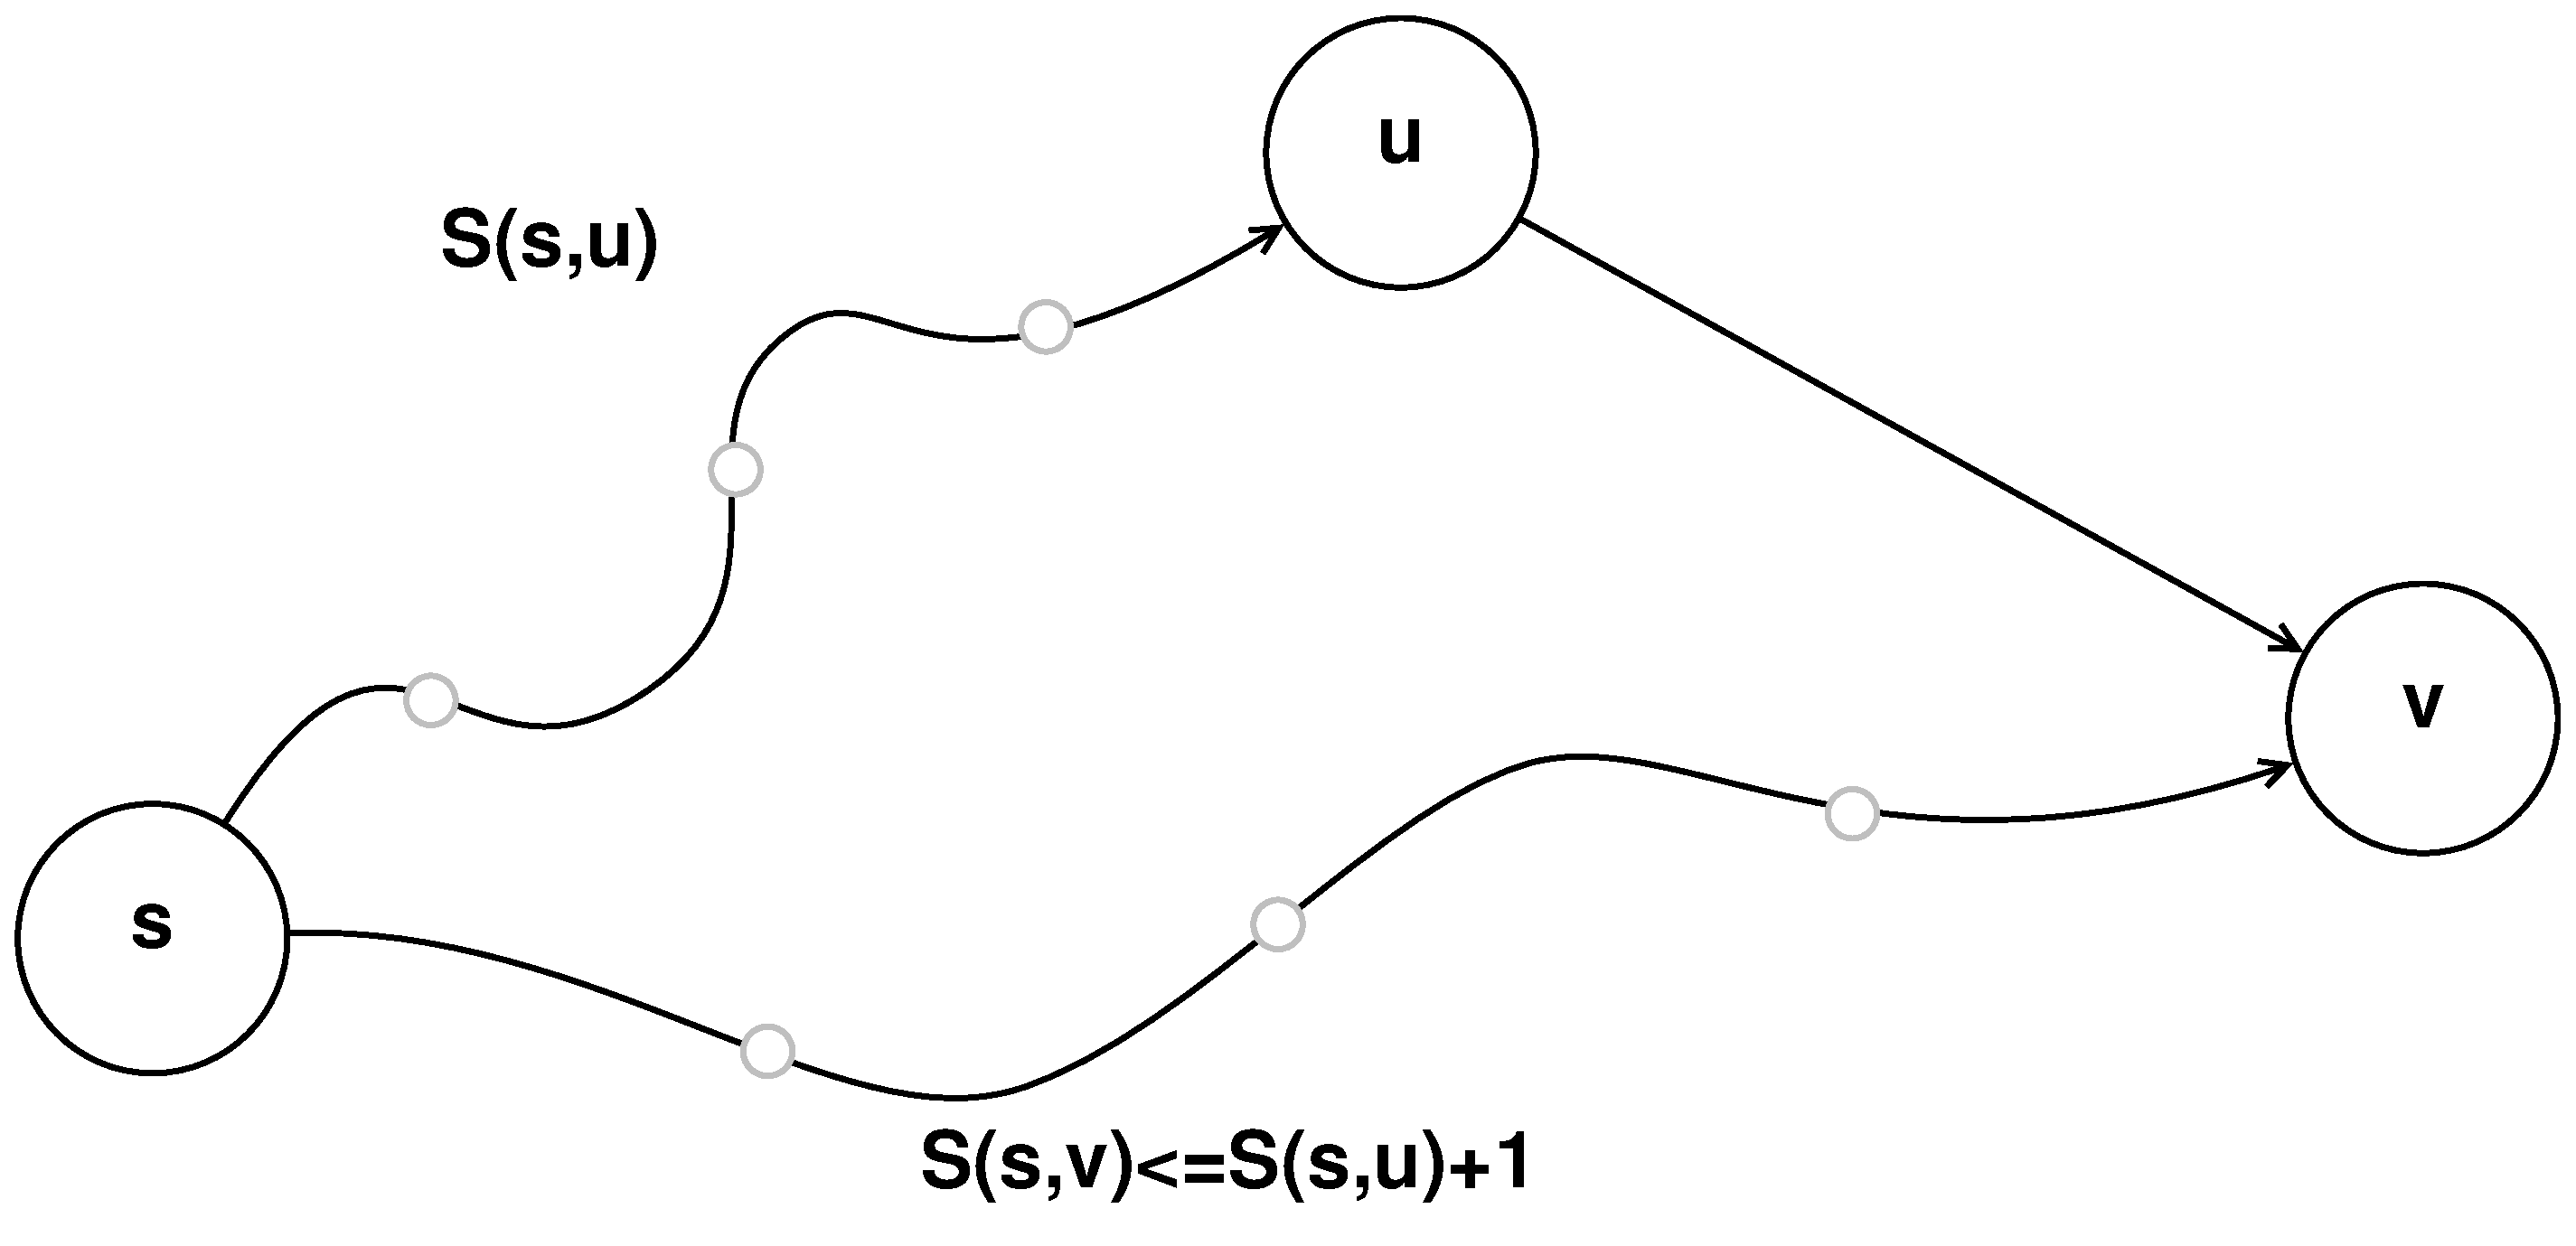
\includegraphics[width=0.7\linewidth]{16/Grafik/Dreiecksungleichung}
\caption{}
\label{fig:Dreiecksungleichung}
\end{figure}

\subsubsection{Lemma 2}
Zu jedem Zeitpunkt im Verlauf von BFS gilt:
\[ \forall v\in V:~ d[v] \geq \delta(s,v)\]
\subsubsection{Beweis (induktiv über Zahl der Operationen, die d-Wert verändern)}
\paragraph{Induktions-Anfang} \[ d[s] = 0 \surd\]
\paragraph{Induktions-Schritt} Knoten $v$ wird von $u$ aus neu entdeckt
\[ d[u]\geq \delta(s,u) \]
\[ d[v] = d[u]+1 \geq \delta(s,u)+1 \overset{D.U.}{\geq} \delta(s,v) \]
\subsubsection{Lemma 3}
Sei $Q=(v_1,v_2,\ldots,v_k)$ eine Queue, dann gilt stets:
\[ d[v_1]\leq d[v_2]\leq\ldots\leq d[v_k]\leq d[v_1]+1 \]
\subsubsection{Beweis (induktiv über die Zahl der push- und pop-Operationen)}
\paragraph{Induktions-Anfang}
\[ d[s] = 0 \surd\]
\paragraph{Induktions-Schritt}
\subparagraph{pop}
\[  \text{\sout{$d[v_1]$}}\leq d[v_2]\leq\ldots\leq d[v_k]\leq d[v_1]+1 \overset{!}{\leq} d[v_2]+1 \]
\subparagraph{push}
\[ d[u] = d[v_1]\leq d[v_2]\leq\ldots\leq d[v_k]\leq d[u]+1 \]
Beachte Kante $(u,v)$ $v$ ist weiß
\[ v=v_{k+1} \text{ wird gepushed} \]
\[ d[v_{k+1}] = d[v_1]+1 \]
Zustand von Q nach push
\[ d[v_2 \leq d[v_3] \leq\ldots\leq d[v_k]\leq d[v_1]+1 = d[v_{k+1}]~~\surd \]
\subsubsection{Satz: Richtigkeit des Algorithmus}
Nach Ablauf von BFS\footnote{Breitensuche} gilt 
\[ \forall v\in V: ~ d[v]=\delta(s,v) \]
\subsubsection{Beweis durch Widerspruch}
Sei $v\in V$, so dass $d[v] \neq \delta(s,v)$ am Ende des Algorithmus $\overset{Lemma2}{\Longrightarrow} d[v] > \delta(s,V)$\\
Sei $v$ so gewählt, dass es der erste knoten ist mit der Eigenschaft, dass sein d-Wert flasch gesetzt wird. d.h. Alle d-Werte bis zu diesem Zeitpunkt sind korrekt.\\
Sei $s\mapsto u'\rightarrow v$ ein kürzester Weg $s$ ui $v$\\
Betrachte die Situation bei Bearbeitung von $u'$:
\paragraph{1. Fall} $v$ ist in diesem Moment schwarz.
\[ d[v] > \delta(s,v)=\delta(s;u')+1\geq\footnote{$v$ vor $u'$ aus $Q$ entfernt und Lemma 3.} d[v]\lightning \]
\paragraph{2. Fall}
$v$ ist in diesem Moment weiß.
\[ d[v]>\delta(s,u')+1=d[u']+1=\footnote{wegen Wahl von $v$; d-Wert von $u'$ muss also korrekt sein}d[v] \lightning \]
\clearpage
\paragraph{3. Fall}
\begin{wrapfigure}{r}{0.4\linewidth}
	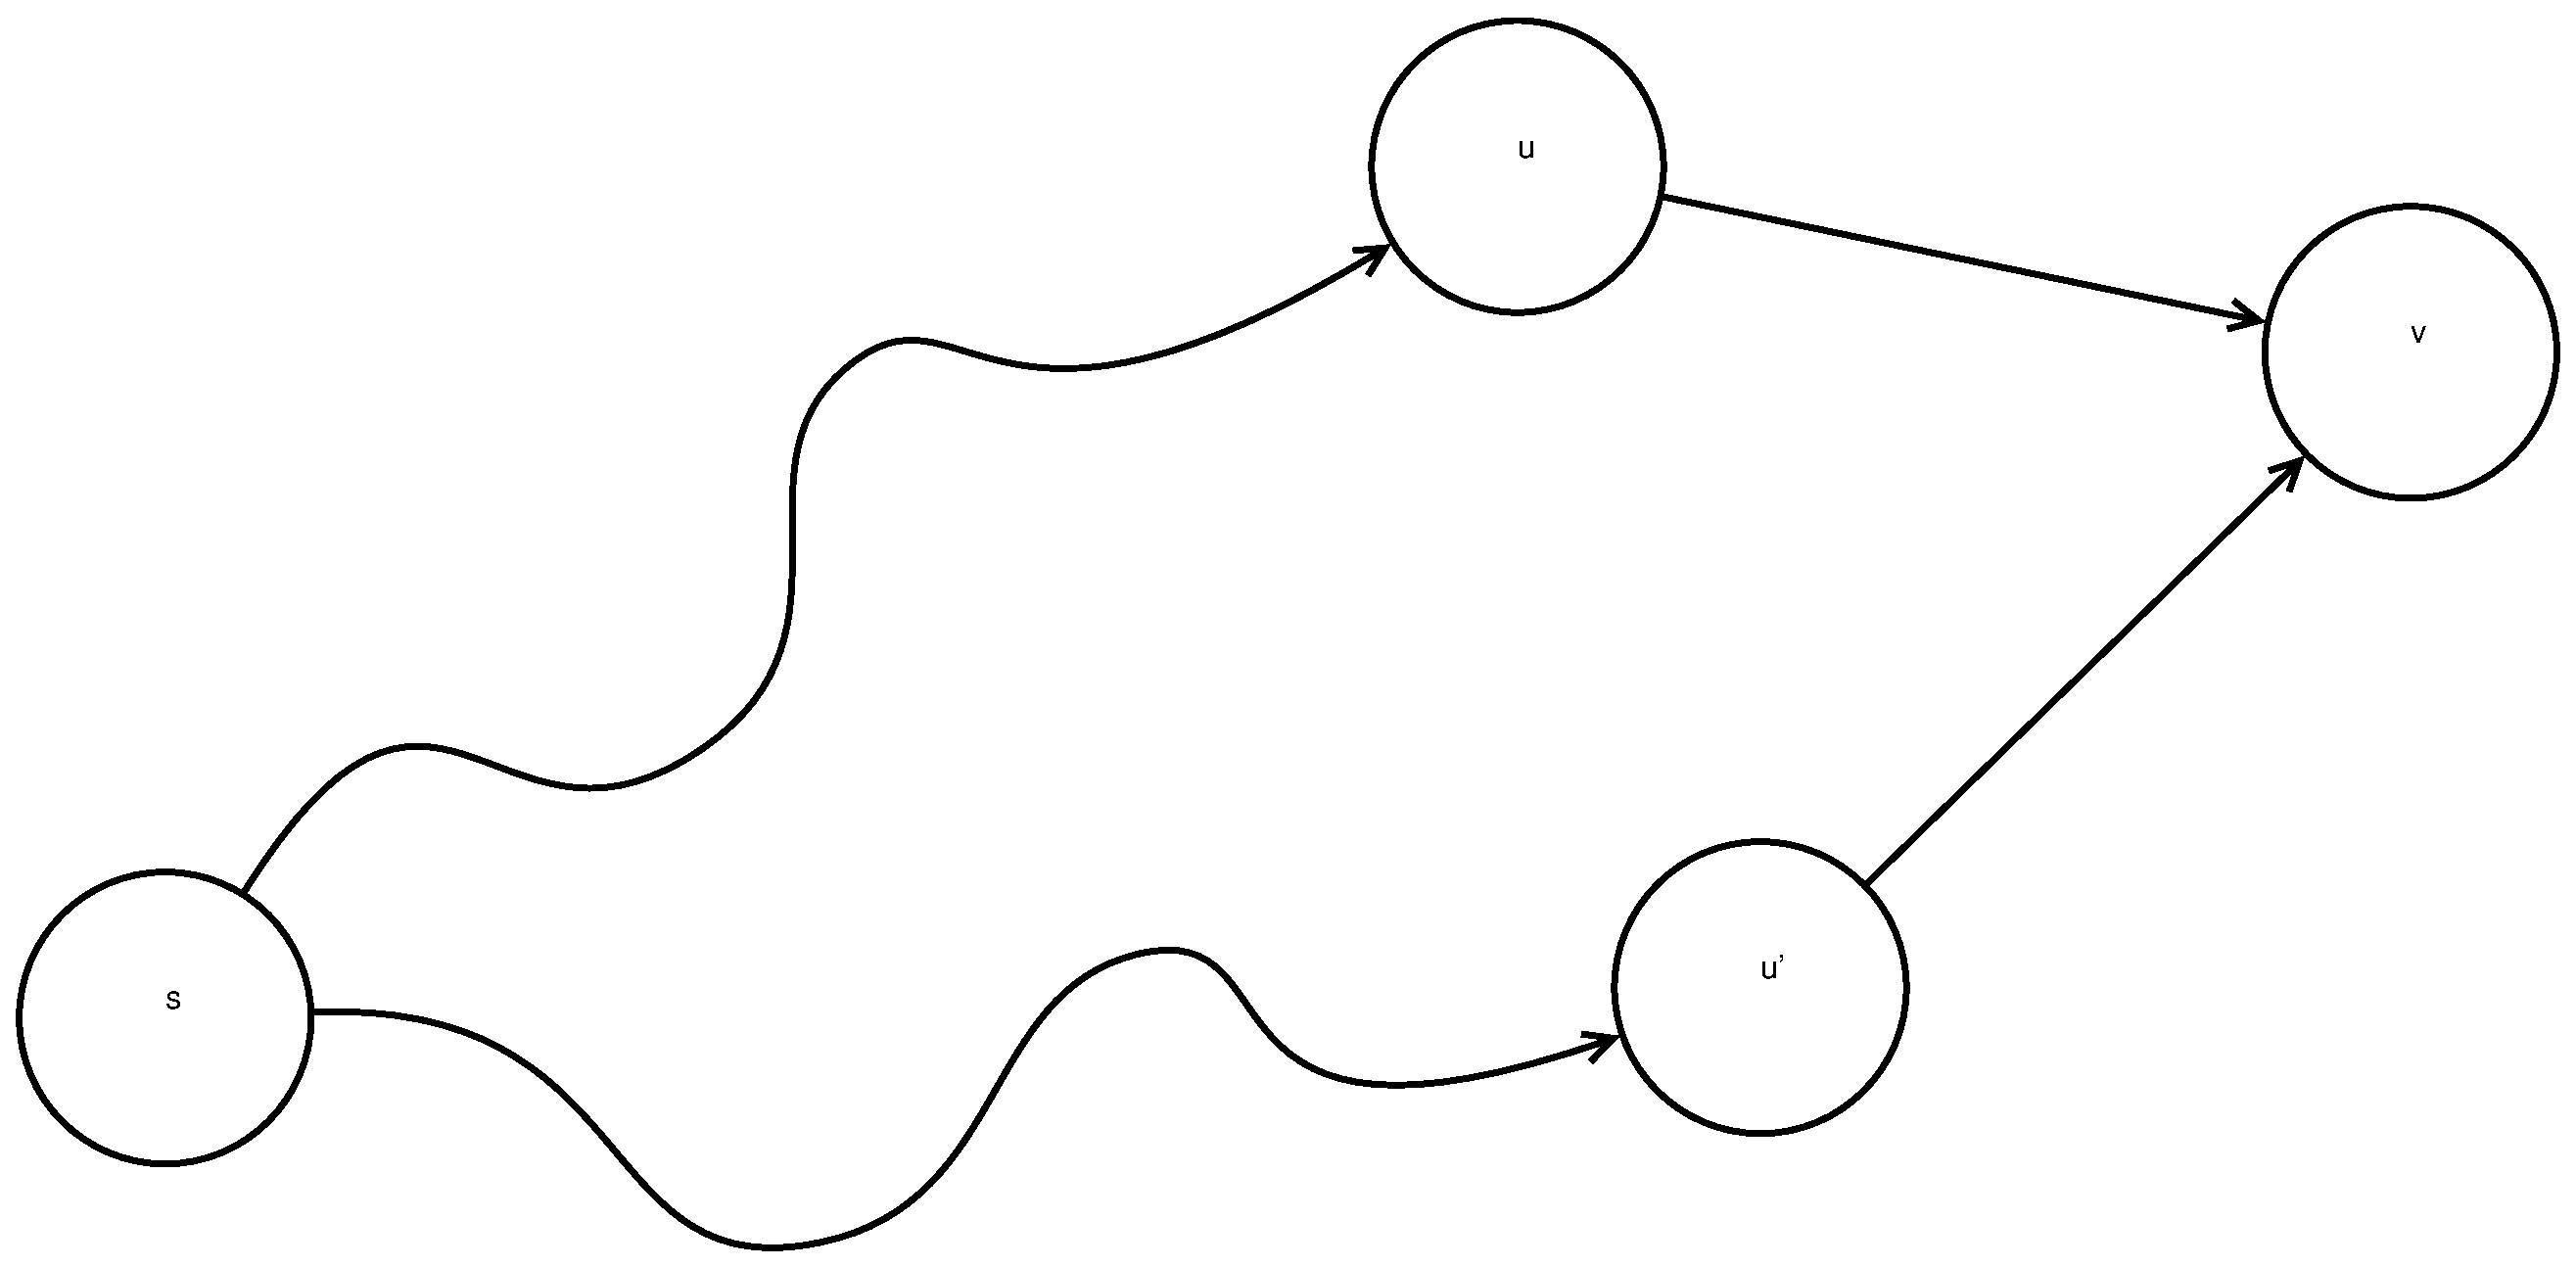
\includegraphics[width=\linewidth]{16/Grafik/Beweis}
	\caption{}
	\label{fig:Beweis}
\end{wrapfigure}
$v$ ist grau.
\[ d[v]>\delta(s,u')+1=d[u']+1\geq d[u]+1=d[v] \]
$d[u]\leq d[u']$, weil $u$ vor $u'$ aus $Q$ entfernt $\lightning$
\begin{flushright}
	q.e.d.
\end{flushright}
\section{Kürzeste Wege Algorithmen}
\section{Dijkstra-Algorithmus}
\[ G=(V,E)~~w:E\rightarrow \mathbb{R}^+_0 \]
\begin{figure}[h]
\centering
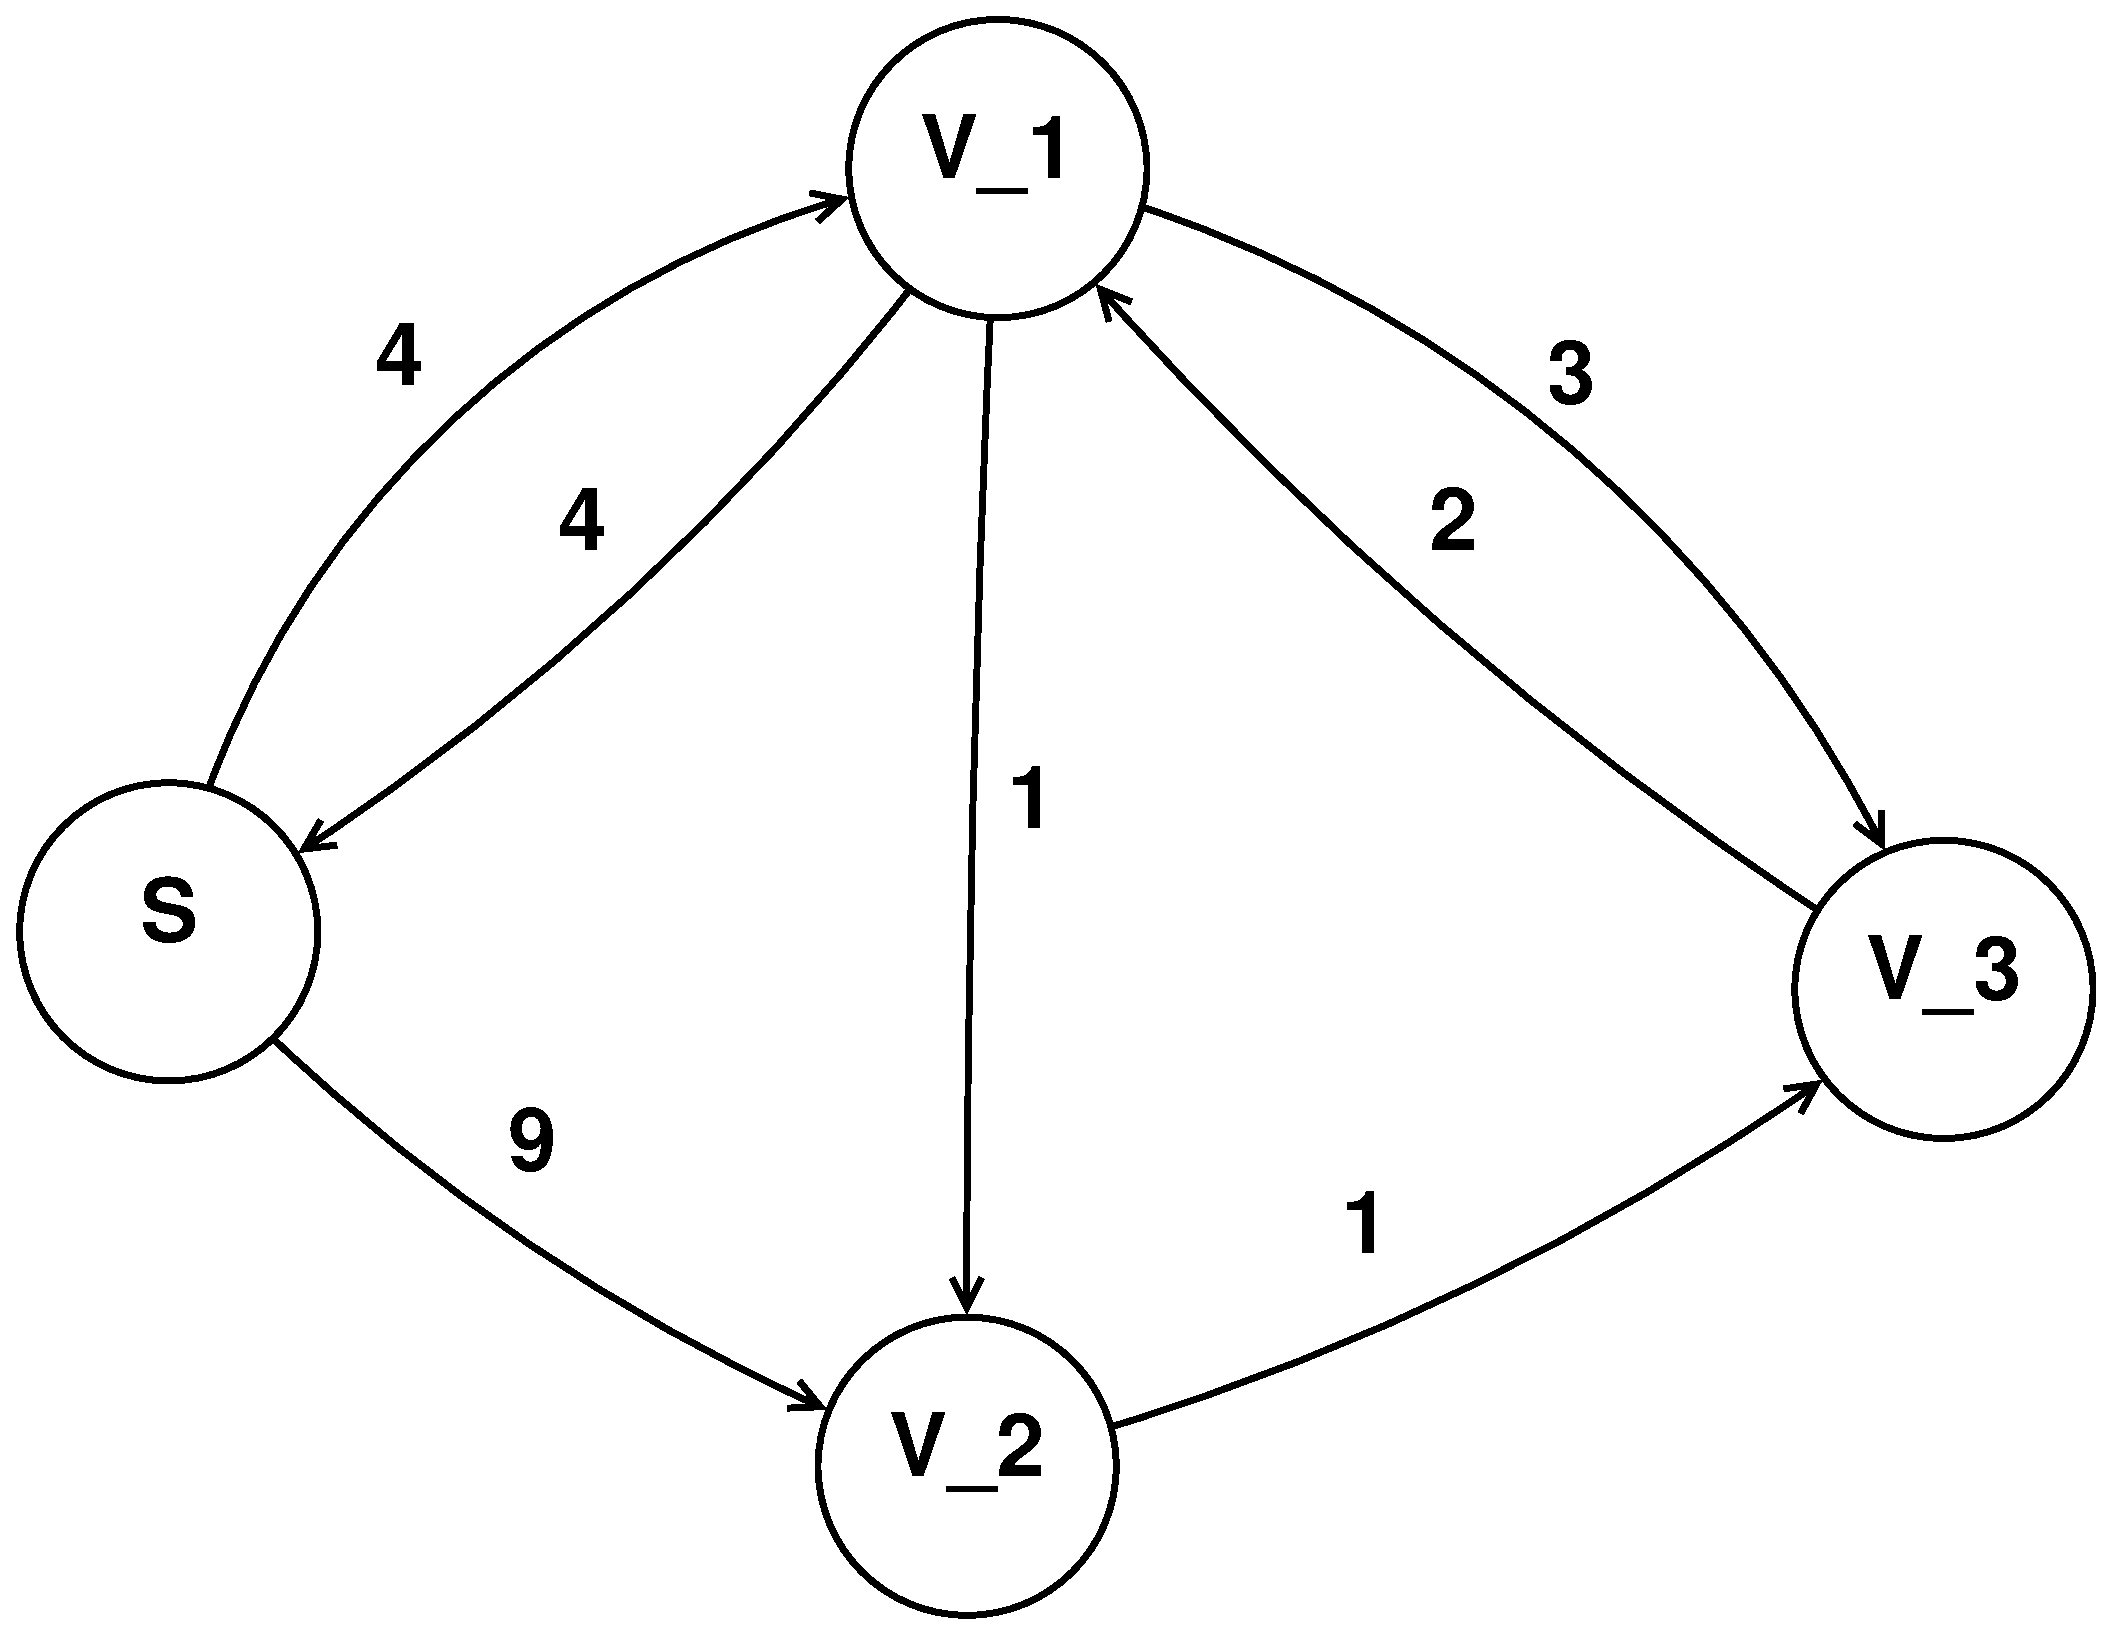
\includegraphics[width=0.3\linewidth]{16/Grafik/Dijkstra}
\caption{}
\label{fig:Dijkstra}
\end{figure}

Sei $p=(s=v_0,v_1,v_2,\ldots,v_k)$
\begin{figure}[h]
	\centering
	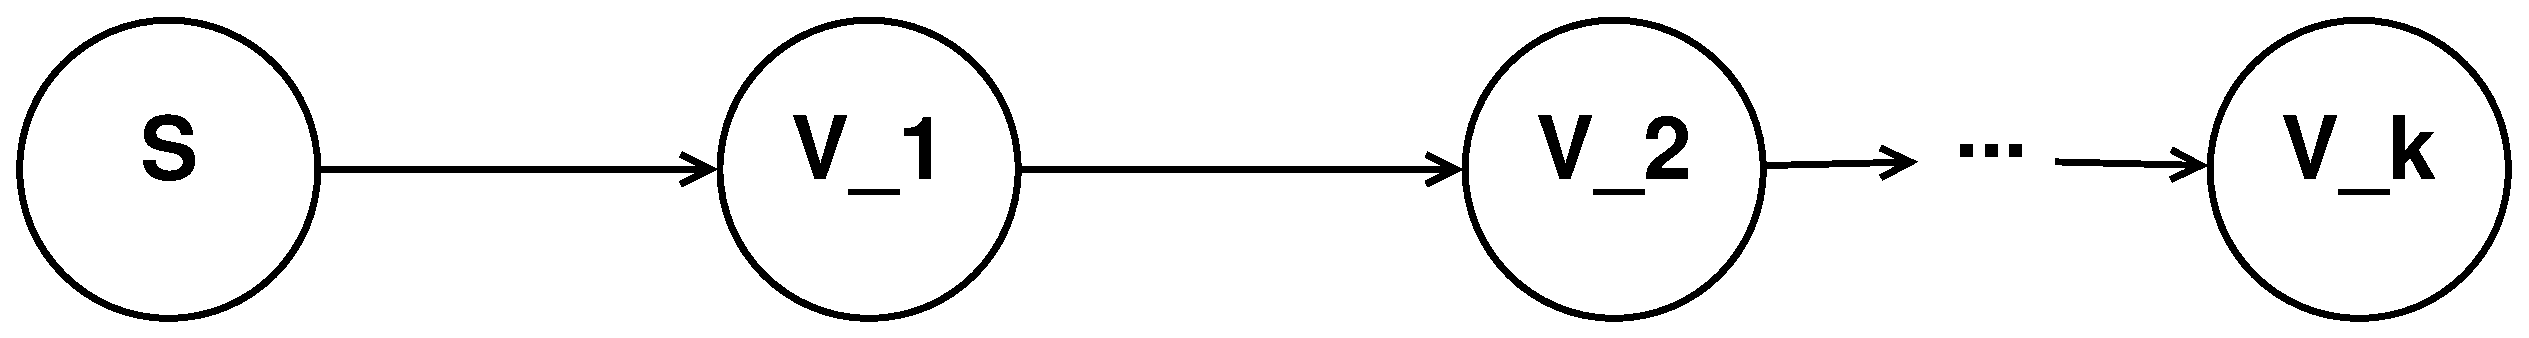
\includegraphics[width=0.3\linewidth]{16/Grafik/Dijkstra2}
	\caption{}
	\label{fig:Dijkstra2}
	\end{figure}
\[ w(p) = \sum_{i=0}^{k-1}w(v_i,v_{i+1})=\delta(s,v_k) \]
\begin{figure}[h]
	\centering
	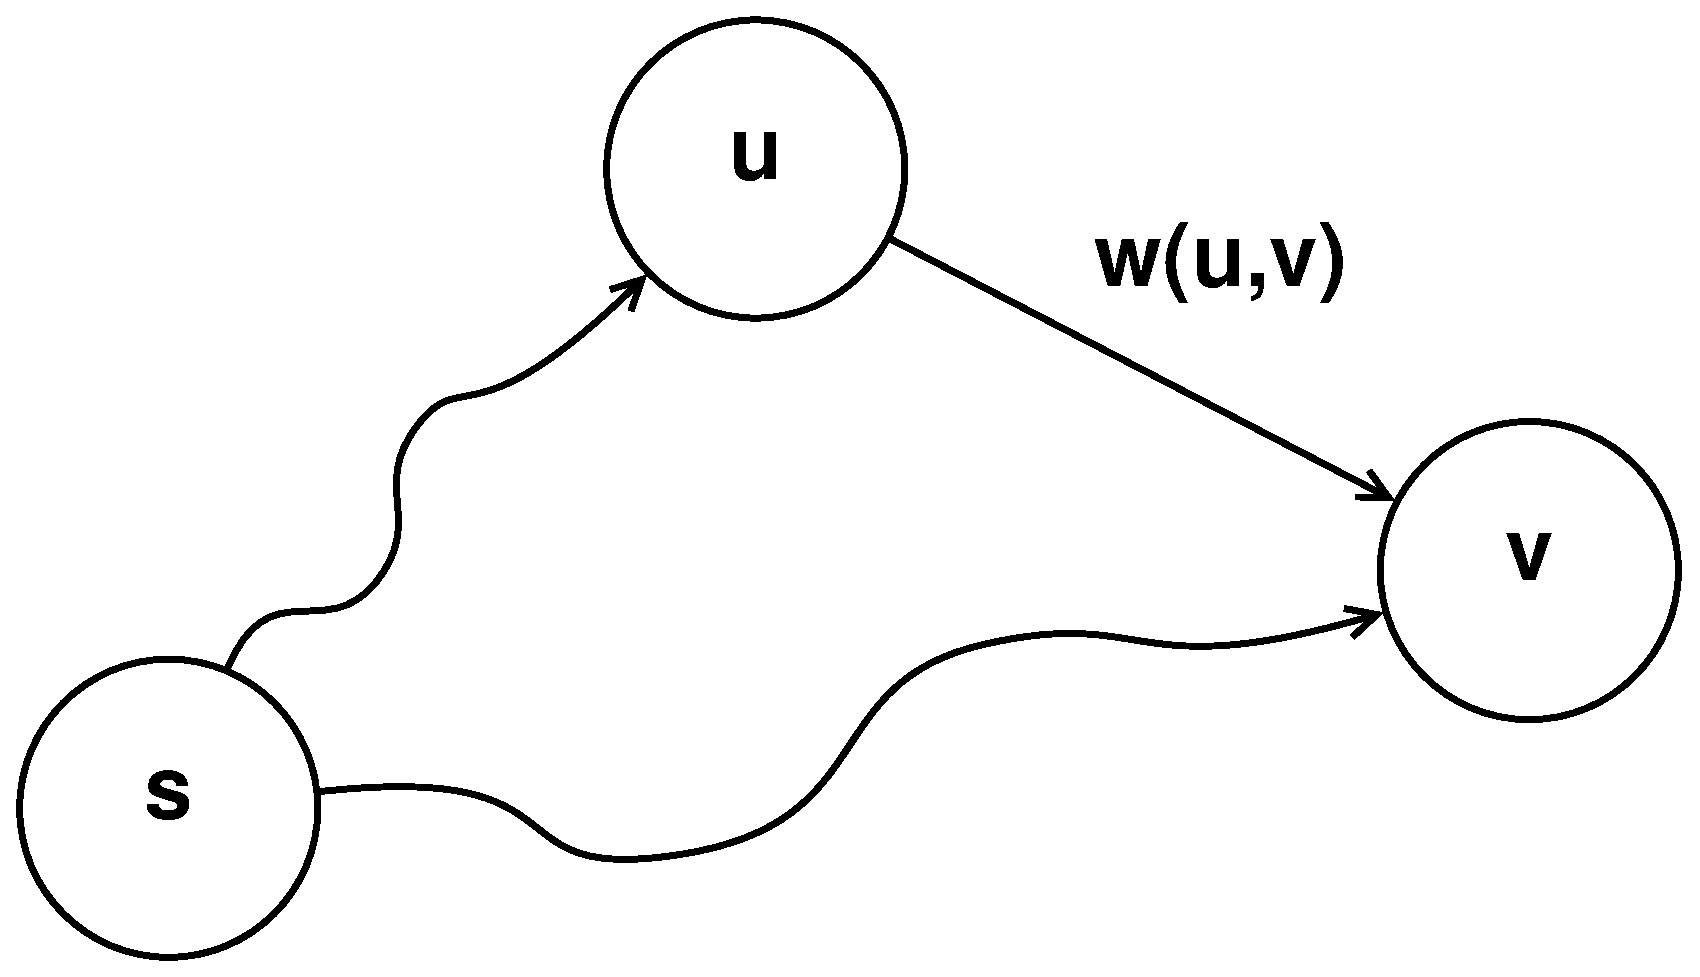
\includegraphics[width=0.3\linewidth]{16/Grafik/dijkstra3}
	\caption{}
	\label{fig:Dijkstra3}
	\end{figure}
\[ \delta(s,v)\leq \delta(s,U)+w(u,v) \]
\begin{lstlisting}
relax(u,v,w) {
  if(d[v] > d[u]+w(u,v) ) {
    d[v] = d[u] + w(u,v);
    /pi[v] = u;
  }
}
\end{lstlisting}
Betrachte Algorithmen zur kürzesten Wege Berechnung, die Distanzwerte nur mit Hilfe dieser relax-Funktion verändern, dann gilt:
\[ d[v] \geq \delta(s,v)~~\forall v\in V \]
\paragraph{Beweis}
\[ d[v] = d[u]+w(u,v) \overset{I.A.}{\geq} \delta(s,u)+w(u,v) \geq \delta(s,v) \]
Induktion über Zahl der reflex-Aufrufe